\section{Analisi della struttura e delle esigenze dell'azienda}

Secondo le informazioni ricevute, l'azienda è costituita da 4 locali:
\begin{itemize}
\item un locale che ospita due server
\item un ufficio per la reception con tre postazioni e una stampante
\item due uffici ognuno con due postazioni una stampante collegati via wireless ad un AP
\end{itemize}
Sono necessari quindi 2 server, 7 postazioni di cui 4 con scheda di rete wireless e 3 stampanti di cui 2 con scheda di rete wireless. Di seguito la rappresentazione grafica dell'azienda. \\
\vspace{40pt}
\begin{figure}[!h]
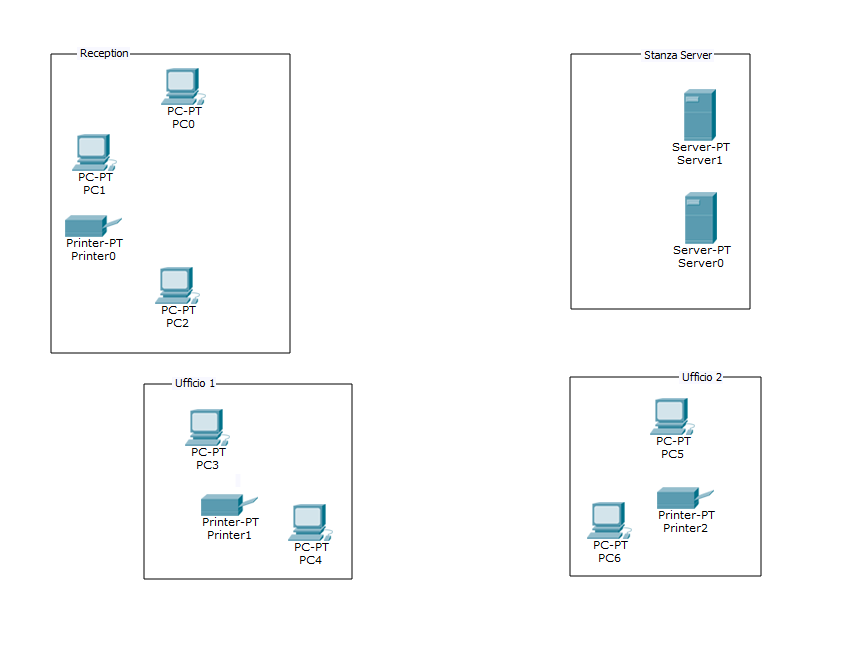
\includegraphics[scale=0.81]{analisi_strutturale}
\label{fig:as1}
\end{figure}
\vspace{40pt}
La rete deve essere efficiente e scalabile, perciò si ha bisogno di cavi e nodi di commutazione che possano soddisfare al massimo queste due richieste.